\documentclass[conference]{IEEEtran}
%\usepackage{enumitem}
\usepackage{framed}
\usepackage{listings}
\usepackage{amstext}
\usepackage{amstext}
\usepackage{pdfpages}
\usepackage{alltt}
\usepackage{epstopdf}
\usepackage{xspace,colortbl}
\usepackage[USenglish]{babel}
\usepackage{multirow}
\usepackage{url}
\usepackage{subfigure}
\usepackage{graphicx}%%
\usepackage{amssymb}
\usepackage{fmtcount}
\usepackage{amsfonts}
\usepackage{xspace}
\usepackage{amsmath}
\usepackage{multirow}
\usepackage[mathscr]{eucal}
\usepackage{times}
\usepackage{colortbl}
\usepackage{bm}
\usepackage[nospace]{cite}

% numbers option provides compact numerical references in the text. 
\usepackage[numbers]{natbib}
\usepackage{multicol}
\usepackage[bookmarks=true]{hyperref}

\pdfinfo{
   /Author (Homer Simpson)
   /Title  (Robots: Our new overlords)
   /CreationDate (D:20101201120000)
   /Subject (Robots)
   /Keywords (Robots;Overlords)
}

\begin{document}

\newtheorem{theorem}{Theorem}
\newtheorem{example}{Example}
\newtheorem{definition}{Definition}
\newtheorem{proposition}{Proposition}
\newtheorem{lemma}{Lemma}
\newtheorem{corollary}{Corollary}

% paper title
\title{Template paper for the \\Robotics: Science and Systems Conference}

% You will get a Paper-ID when submitting a pdf file to the conference system
\author{Author Names Omitted for Anonymous Review. Paper-ID [add your ID here]}

%\author{\authorblockN{Michael Shell}
%\authorblockA{School of Electrical and\\Computer Engineering\\
%Georgia Institute of Technology\\
%Atlanta, Georgia 30332--0250\\
%Email: mshell@ece.gatech.edu}
%\and
%\authorblockN{Homer Simpson}
%\authorblockA{Twentieth Century Fox\\
%Springfield, USA\\
%Email: homer@thesimpsons.com}
%\and
%\authorblockN{James Kirk\\ and Montgomery Scott}
%\authorblockA{Starfleet Academy\\
%San Francisco, California 96678-2391\\
%Telephone: (800) 555--1212\\
%Fax: (888) 555--1212}}


% avoiding spaces at the end of the author lines is not a problem with
% conference papers because we don't use \thanks or \IEEEmembership


% for over three affiliations, or if they all won't fit within the width
% of the page, use this alternative format:
% 
%\author{\authorblockN{Michael Shell\authorrefmark{1},
%Homer Simpson\authorrefmark{2},
%James Kirk\authorrefmark{3}, 
%Montgomery Scott\authorrefmark{3} and
%Eldon Tyrell\authorrefmark{4}}
%\authorblockA{\authorrefmark{1}School of Electrical and Computer Engineering\\
%Georgia Institute of Technology,
%Atlanta, Georgia 30332--0250\\ Email: mshell@ece.gatech.edu}
%\authorblockA{\authorrefmark{2}Twentieth Century Fox, Springfield, USA\\
%Email: homer@thesimpsons.com}
%\authorblockA{\authorrefmark{3}Starfleet Academy, San Francisco, California 96678-2391\\
%Telephone: (800) 555--1212, Fax: (888) 555--1212}
%\authorblockA{\authorrefmark{4}Tyrell Inc., 123 Replicant Street, Los Angeles, California 90210--4321}}


\maketitle

\begin{abstract}
TODO
\end{abstract}

\section{Introduction}
Large datasets can be prone to error \cite{Gartner}, and data cleaning has been studied to mitigate query error on dirty data \cite{dasu2003exploratory, mayfield2010eracer, openrefine, wrangler, DBLP:conf/sigmod/DallachiesaEEEIOT13, DBLP:conf/pervasive/JefferyAFHW06}.
An important subclass of data cleaning problems are Entity Resolution (ER) problems which have had much research interest both historically and recently. \cite{DBLP:journals/pvldb/KopckeTR10, conf/dmkd/MongeE97, conf/sigmod/WhangMKTG09, conf/acl/FinkelM08, conf/sigmod/WangLF12, Fellegi1969, conf/sigmod/ArasuGK10, DBLP:journals/tkde/ElmagarmidIV07, journals/tkde/Christen11, getoor2005link}
In these problems, for every record we want to find a single canonical mapping between the record and a real-world entity.
This includes regularizing representations, removal of duplicate records, and removal of irrelevant records.

A popular theoretical model for ER is the functional dependency model.
The concept of a functional dependency has been well studied in the database literature 
and was proposed by Codd in 1974 \cite{codd1974recent}.
Recent work explores encoding ER primitives as types of functional dependencies called Conditional Functional Dependencies (CFD) \cite{bertossi2013data, fan2014interaction, fan2008conditional}.
These are basically rules that encode unsatisfied constraints based on expert input (i.e NY == New York) and the data cleaning algorithm iterates until these constraints are satisfied.
As this formulation fits nicely into a Satisfiability-like framework, many theoretical insights have naturally followed such determining the minimal sequence of data changes to satisfy all of the constraints is coNP-Hard. \reminder{SK: todo clarify section}

As the coNP-Hard result suggests, while this model gives insights into what types of errors occur in a dataset, there is a challenge of efficiently repairing the errors (i.e. enforcing the constraints).
Bertossi et al. \cite{bertossi2013data} found that a lattice data structure could be used to a find PTIME iterative algorithm for ER problems with only ``matching" dependencies.
Wang et al. \cite{wang2014towards} extended the CFD framework with ``fixing" rules; rules that also prescribed fixes which as in Bertossi et al. makes the cleaning algorithms faster and more reliable.

A key assumption of the functional depedency work in data cleaning has been \emph{infallible} rules.
However, in practice, this is rarely the case.
Large datasets are often pre-processed with chains of heuristic data cleaning operations each with their own precision and recall characteristics as in ETL tools \cite{herzog2007data}.
Furthermore, increasingly data cleaning is part of a larger pipeline including streaming, machine learning, or exploratory data analysis.
In this setting, semantics on partial or sampled results are important, and the CFD model may not be appropriate to describe these applications.

In this work, we explore robust execution of \emph{pipelines} of data cleaning operations with an application to ER.
In contrast to prior work, we formalize ER as an algebra over relations as opposed to constraints on tuples in those relations.
A key piece of this work is a data structure we call a \emph{proposal} which propagates an augemnted intermediate state of the pipeline mitigating some times of errors.
We show that in the case where our operations are \emph{infallible}, our formalization naturally leads to the algorithm proposed by Bertossi et al., and exactly the same result with a connected components algorithm over a graph of linked tuples.
However, the connected components version is robust to transitivity errors in the rules which correspond to missing edges in the graph.
We then devise an alternative to the connected components, accounting for spurious edges, using correlation clustering which seperates the graph into components that are approximately cliques.
Finally, we merge proposal data structures from different executions allowing us to try different permutations of the ER pipeline and take a consensus of their results.










\section{Background and Main Ideas}

This section describes the key idea of SampleClean, namely, that data cleaning can be integrated with approximate query processing leading to bounded approximations of clean query results for a fraction of the cleaning cost.

\iffalse
\subsection{Data Cleaning is Often Expensive}
A number of surveys report that data cleaning is one of the most time consuming steps \cite{kandel2012enterprise, nytimes}.
Data cleaning frameworks have been recently proposed to address the problem of corrupted data at scale\cite{khayyat2015bigdansing, chu2015katara, sampleclean}.
As errors can be domain- or dataset-specific, data cleaning is an inherently human-driven process and can require a significant amount of developer effort in writing software or rules to fix the corruption.
Automated fixes may not be reliable and can require human confirmation \cite{DBLP:journals/pvldb/YakoutENOI11}.
One way to scale up human computation is crowdsourcing which has shown recent success in entity resolution and value filling \cite{gokhale2014corleone, park2014crowdfill, sampleclean,chu2015katara}.
However, crowdsourcing comes with the costs of significant additional latency (orders of magnitude slower than data processing) and the overhead of managing human workers.
\fi

\subsection{Traditional Approximate Query Processing}
A number of approximation schemes have been proposed including using Sampling, Wavelets, Sketching, and Hashing (see Cormode et al. for a survey \cite{DBLP:journals/ftdb/CormodeGHJ12}).
This article focuses on Sampling-based approximations and we will use the term AQP to refer to such systems (e.g., BlinkDB\cite{DBLP:conf/eurosys/AgarwalMPMMS13}).
Sampling-based approximate query processing is a powerful technique that allows for fast approximate results on large datasets. 
It has been well studied in the database community since the 1990s~\cite{DBLP:conf/sigmod/HellersteinHW97,DBLP:conf/sigmod/AcharyaGPR99,DBLP:conf/icde/OlkenR92, OlkenR86}, and methods such as BlinkDB~\cite{DBLP:conf/eurosys/AgarwalMPMMS13} have drawn renewed attention in recent big data research. 
An important aspect of this work is confidence intervals, as many types of aggregates can be bounded with techniques such as concentration inequalities (e.g., Hoeffding bounds), large-deviation inequalities (e.g., Central Limit Theorem), or empirically (e.g., Bootstrap). 
Suppose, there is a relation $R$ and a uniform sample $S$.
AQP applies a query $Q$ to $S$ (possibly with some scaling $c$) to return an estimate: 
\[
Q(R) \approx est = c \cdot Q(S)
\]

Traditionally, AQP sacrifices accuracy due to sampling for improved query latency.
However in AQP, the bounds on $est$ assume that the only source of error is approximation error introduced by sampling, however, the data itself may contain errors which could also affect query results.
When the data itself is erroneous, a query result on the full data--let alone a sample, will be incorrect.
The main argument for SampleClean is that when data errors significantly affect query results,
sampling can be combined with data cleaning to actually improve accuracy.
This leads to a counter-intuitive result where it is possible that a query on a cleaned sample of data is more accurate than a query on the entire dirty data.

\iffalse
\subsection{Exploiting Application Structure}

\jn{It's a little too early to present the content of this section before showing the big idea. I would suggest to put it either to the end of Sec 2 or the end of Sec 3. }

SampleClean applies sample to clean $k\ll N$ rows in a database to address the time-scale mismatch between the analytics application (e.g., SQL query, Machine Learning, Materialized View) and data cleaning.
An important aspect of this project is how the structure and semantics of that application can be used to prioritize and budget data cleaning.
A database only needs to be sufficiently clean for the requirements of the subsequent analytics--and the key insight from AQP being that aggregates are tolerant to approximation.

In the initial SampleClean work, we restricted the allowed aggregate queries to \sumfunc, \countfunc, and \avgfunc with predicates and group by clauses.
In the two subsequent projects, View Cleaning and ActiveClean, we expanded the scope and the semantics of the application. 
The View Cleaning problem explores data cleaning and general aggregates on derived relations with known view definitions.
We can exploit view definition to query just as much of the base data as needed to accurately answer the aggregate query for a fixed budget.
In fact, we showed that any aggregate (beyond \sumfunc, \countfunc, and \avgfunc) that could be estimated with AQP\cite{agarwalknowing}, could be answered estimated with the View Cleaning framework.
ActiveClean generalizes the initial work on \sumfunc, \countfunc, and \avgfunc to higher-dimensional aggregates.
We defined a class of analytics called Convex Data Analytics, and show how the convex structure of the analytics can be used to guide and prioritize data cleaning.
\fi

\subsection{Approximate Query Processing on Dirty Data}


\subsubsection{Two Sources of Errors: Sampling Error and Data Error}
If $R$ is dirty, then there is a true relation $R_{clean}$.
\[
Q(R_{clean}) \ne Q(R) \approx est = c \cdot Q(S)
\]
The error in $est$ has two components: error due to sampling $\epsilon_s$ and error due to the difference with the cleaned relation $\epsilon_c = Q(R_{clean}) - Q(R)$:
\[
\mid Q(R_{clean}) - est \mid \le \epsilon_s + \epsilon_c
\]

While they are both forms of query result error, $\epsilon_s$ and $\epsilon_c$ are very different quantities.
$\epsilon_s$ is a random variable due to the sampling, and different samples would result in different realizations of $\epsilon_s$.
As a random variable introduced by sampling, $\epsilon_s$ can be bounded by a variety of techniques as a function of the sample size.
On the other hand, $\epsilon_c$ is deterministic, and by definition is an unknown quantity until all the data is cleaned.
Thus, the bounds returned by a typical AQP framework on dirty data would neglect $\epsilon_c$.

It is possible that $R_{clean} \ne R$ but $\epsilon_c=0$.
Consider a \sumfunc query on the relation $R(a)$, where $a$ is a numerical attribute.
If half of the rows in $R$ are corrupted with $+1$ and the other half are corrupted with $-1$, then $Q(R_{clean}) = Q(R)$.
The interesting problem is when there are \emph{systematic errors}\cite{taylor1982introduction} i.e., $\mid \epsilon_c \mid > 0$. 
In other words, the corruption that is correlated with the data, e.g., where every record is corrupted with a $+1$.

\subsubsection{Key Idea I: Direct Estimate vs. Correction}
The key quantity of interest is $\epsilon_c$, and to be able to bound
a query result on dirty data, requires that $\epsilon_c$ is 0 or bound $\epsilon_c$.

\vspace{0.5em}
\noindent\textbf{Direct Estimate: } This technique is a direct extension of AQP to handle data cleaning. A set of $k$ rows is sampled uniformly at random from the dirty relation $R$ resulting in a sample $S$. Data cleaning is applied to the sample $S$ resulting in $S_{clean}$.
Data cleaning and sampling may change the statistical and scaling properties of the query $Q$, so $Q$ may have to be re-written to a query $\widehat{Q}$. $\widehat{Q}$ is applied to the sample $S_{clean}$ and the result is returned. 
There are a couple of important points to note about this techniques.
First, as in AQP, the direct estimate only processes a sample of data.
Next, since it processes a cleaned sample of data, at no point is there a dependence on the dirty data.
As we will show later in the article, the direct estimate returns a result whose accuracy is independent of the magnitude or rate of data error. 
One way to think about this technique is that it ensures $\epsilon_c = 0$ within the sample.

\vspace{0.5em}
\noindent\textbf{Correction: } The direct estimate suffers a subtle drawback. Suppose, there are relatively few errors in the data. The errors introduced by sampling may dominate any error reductions due to data cleaning. As an alternative, we can try to estimate $\epsilon_c$. A set of $k$ rows is sampled uniformly at random from the dirty relation $R$ resulting in a sample $S$. Data cleaning is applied to the sample $S$ resulting in $S_{clean}$. 
The difference in applying $\widehat{Q}$ to S and $\widehat{Q}$ to $S_{clean}$ gives an estimate of $\epsilon_c$. 
The interpretation of this estimate is a correction to the query result on the full dirty data.
In contrast to the direct estimate, this technique requires processing the entire dirty data (but only cleaning a sample).
However, as we will later show, if errors are rare this technique gives significantly improved accuracy over the direct estimates.

\subsubsection{Key Idea II: Sampling to Improve Accuracy}
%A small sample of clean data can improve query accuracy.
Figure \ref{fig:est2} plots error as a function of the cleaned sample size on a corrupted TPCH dataset for a direct estimate, correction, and AllDirty (query on the full dirty data).
In both cases, there is a break-even point (in terms of number of cleaned samples) when the data cleaning has mitigated more data error than the approximation error introduced by sampling.
After this point, SampleClean improves query accuracy in comparison to AllDirty.
When errors are relatively rare (5\% corruption rate), the correction is more accurate. 
When errors are more significant (50\% corruption rate), the direct estimate is more accurate.
Note that the direct estimate returns results of the same accuracy regardless of the corruption rate. 

\begin{SCfigure}
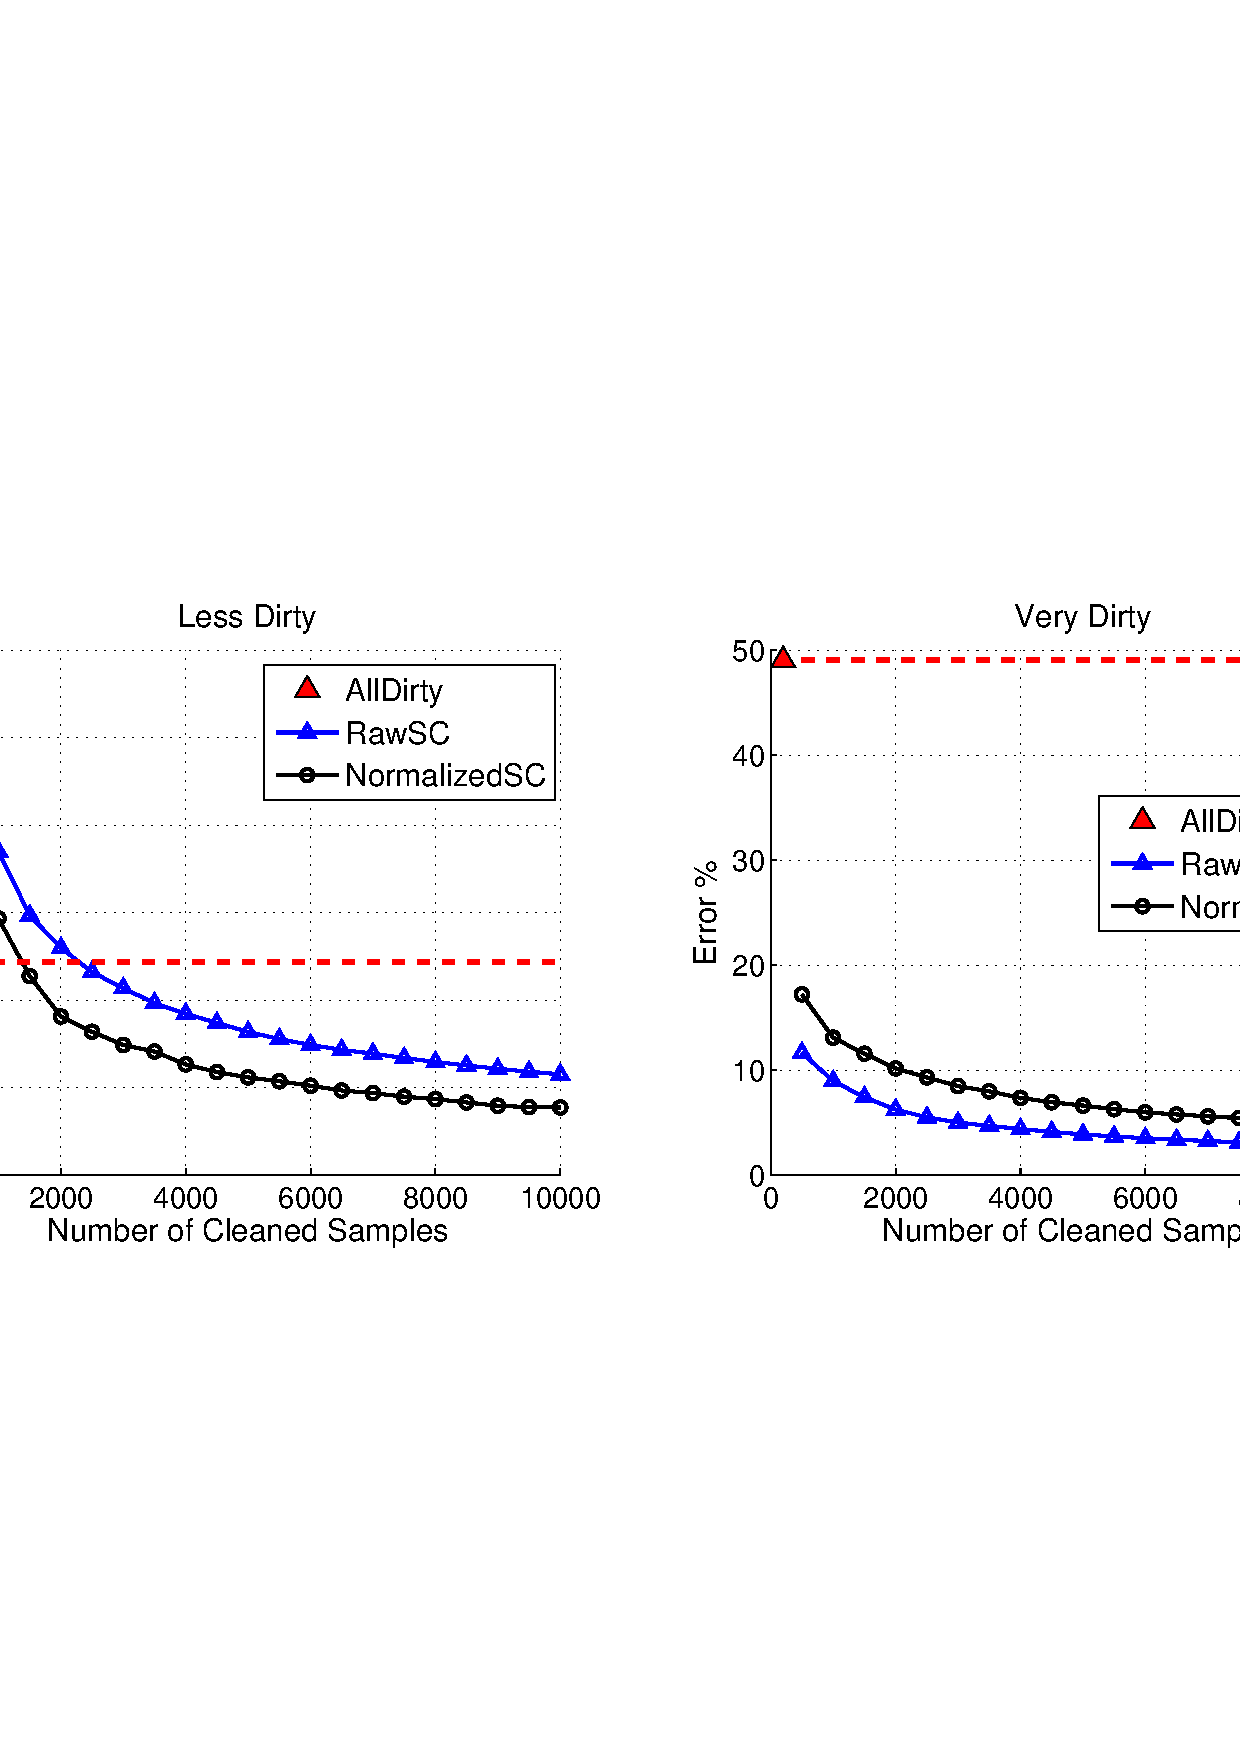
\includegraphics[width=.6\columnwidth]{figs/allerror-samplesize.pdf}
\caption{Comparison of the convergence of the methods on two TPC-H datasets of 6M tuples with simulated errors 50\% error and 5\% error. On the dataset with larger errors, the direct estimate gives a narrower confidence interval, and on the other the correction is more accurate. \label{fig:est2}}
\end{SCfigure}




\section{Beta Process Models For Segmentation}
The Beta-Bernoulli model is a Bayesian non-parametric approach to assign 
a set of observations to a set of features [cite].
One of key aspects of this approach is it allows for clustering with \emph{mult-tenancy}; 
that is observations may be members of multiple clusters.
This approach has been applied the segmentation of dynamical trajectories [cite], however,
has not yet been applied to identify kinematic primitives.

The kinematic case poses a variety of new challenges.
First, we need to explictly make the model invariant to rotations.
The next challenge is that kinematic primitives are more sensitive to
time scales and thus we need to be careful with how we model the windowing operations
and how those windows are allowed to interact with other properties such as rotation invariance.

The standard recipe for Bayesian approaches is to define a generative model; a plausible parameterized statistical model
that generates the observed data.
Then conditioned on the observations infer the expected model.

\textbf{SK: The notation below is inconsistent with the stuff I added}
\subsection{Generative Model For Demonstration-Trajectory Relationship}
We first look at the case for fixed $K$ number of motion primitives.
In this case, we assume the demontration are created by the following
generative model for each demonstration $i$:
\begin{enumerate}
\item Draw $T_{i}\sim Poisson(\gamma)$
\item Draw $\theta\sim Beta(\alpha)$
\item Draw $R\sim N(I,\sigma I)$
\item For $1..t..T_{i}$

\begin{enumerate}
\item For 1..k..K

\begin{enumerate}
\item Choose $z_{ik}\sim Ber(\theta)$ 
\end{enumerate}
\item $\tau_{i}[t]=R(\sum_{k}z_{ik}p_{k})+\epsilon$
\item $\epsilon\sim N(0,\sigma I)$
\end{enumerate}
\end{enumerate}
Now, if we allow $K\rightarrow\infty$, that is a potentially infinite
number of primitives, this model becomes a Beta Process model:
\begin{enumerate}
\item Draw $T_{i}\sim Poisson(\gamma)$
\item Draw $B\sim BP(1,B_{0})$
\item Draw $R\sim N(R_{0},\sigma I)$
\item For $1..t..T_{i}$

\begin{enumerate}
\item $Z\sim BeP(B)$ 
\item $\tau_{i}[t]=R(\sum_{k}^{\infty}Z_{ik}p_{k})+\epsilon$ 
\item $\epsilon\sim N(0,\sigma I)$
\end{enumerate}
\end{enumerate}
Due to the isotropic nature of the generative model, this can be solved
using a variant of BP-Means proposed by Broderic, Kulis, and Jordan
2012 {[}cite{]}. \{TODO: A relaxation is needed to make the translation
invariance work\}


\subsection{Parameter Inference For $\mathbb{P}$}

As in {[}cite{]}, let $1...K^{+}$ index the current set of primitives
$\mathbb{P}$.
\begin{enumerate}
\item For all demonstrations

\begin{enumerate}
\item Calculate expected $R$: via orthonormally constrained least squares
(as in Mahler et al.) fit a rigid transformation to all $\tau\in x_{i}$,$p\in\mathbb{P}$
and take the mean.
\item For all trajectories within a demonstration

\begin{enumerate}
\item Choose subset of primitives that sum to $\tau$
\item Add current trajectory to set of primitives, if it improves the objective
by more than $\lambda^{2}$ then include it else drop it.
\end{enumerate}
\item Update set of primitives via least squares.\end{enumerate}
\end{enumerate}
\section{Results}
Use three datasets for which we have some ground truth. They are all small

Comparison: Pr* (Optimal single pipeline), RPr (All samples of EPS), RPr-50 (50\% of EPS samples), Pr- (worst pipeline), and baseline* (Jiannan's Crowder Clustering algorithm but using the best sequence of actions).

\subsection{Does Randomization Make Pipelining More Robust?}
Compare to best single pipeline, worst single pipeline, and current state of the art.
We should find that a randomized execution is much better than the worst and hopefully comparable to the best.
In some cases, it may be better than the best, but it should never be worse than the worst.

Dataset: MS Academic 
Operations: Filter and Deduplicate

Dataset: Yelp 
Operations: String Clean, City Format, Deduplicate

Dataset: Product 
Operations: identify sku if exists, string clean, Deduplicate

\begin{figure}[ht]
\centering
\includegraphics[scale=0.4]{fig1.png}
\caption{}
\label{exp:ms-academic-ranking}
\end{figure}

\subsection{How does this vary with random error in the operators?}
Should show that the more unreliable the data cleaning is the more that our approach benefits.

Introduce varying amount of random error (hashed so consistent between runs) into the ``city formatting" fix for the yelp dataset:

\begin{figure}[ht]
\centering
\includegraphics[scale=0.5]{fig2.png}
\caption{}
\label{exp:ms-academic-ranking}
\end{figure}

Introduce varying amount of random error (hashed so consistent between runs) into an extra dedup operation.

\begin{figure}[ht]
\centering
\includegraphics[scale=0.5]{fig3.png}
\caption{}
\label{exp:ms-academic-ranking}
\end{figure}

\subsection{Runtime-Accuracy Tradeoff}
Execute more samples and show how the accuracy improves.

\begin{figure}[ht]
\centering
\includegraphics[scale=0.5]{fig4.png}
\caption{}
\label{exp:ms-academic-ranking}
\end{figure}


\subsection{Large-scale experiments}
Streaming correlation clustering. Show that at scale this technique can work and in a distributed environment.
In order to quantify the robustness of our methodology, we intend to run the algorithm on both synthetic and realworld datasets.
The synthetic dataset give us the ability to control the parameters while explore the state of possible responses.
However, a pitfall with such analysis is it's rather difficult to measure actual improvement over random fluctuations as well as the improvement may not be uniform across all tasks.
With experimentation on the real world datasets, we indent to first show the applicability of our method; and secondly determine whether results from our previous analysis extends to non-synthetic scenarios.




%\section{Related Work}

%% In the context of recommender systems, social influence has been studied primarily in order to use information about social and trusted friend networks to improve recommendations. Jamali et al. described a stochastic block model which predicts recommendations based on both social relations and rating behavior [A]. Shang et al. described models for for improving recommendations among individuals using the theory of social contagion, and among groups using network theory [B]. Ye et al. proposed a quantification metric of social influence, and proposed probabilstic model to model the decision of item selection [C].

%% However, the Asch model for confirmity suggest a particular biasing effect from an aggregate or ``crowd'' (i.e. the previous raters are anonymous to the current rater). This phenomenon known as social herding ...
In their seminal 2003 work, Cosley, Lam, Albert, Konstan, and Reidl \cite{cosley2003seeing} studied the broad problem of biases in rating systems and tested the following relevant hypotheses:  can manipulated ``predicted" ratings influence a participant to change their rating, how consistent participants when re-rating an item, and how does rating scale (eg. stars, binary, unary) affect the average rating. 
The seminal result from Cosley et al. is that all of these hypotheses yielded significant influencing tendencies.
In this paper, we formulate a predictive model for a specific type of bias, social influence bias, which is learned and isolated through the unique interface of the CRC. 
We also apply a nonparametric significance testing methodology.

The Asch model for conformity is the theoretical basis for what is sometimes called \emph{social herding}, the tendency to conform \cite{banerjee1992simple,bikhchandani2000herd}, and this is a well-known choice model in economics \cite{burnkrant1975informational,dholakia2002auction,huang2006herding}. 
Such models have also been studied in psychology and behavioral economics as ``persuasion bias" \cite{demarzo2003persuasion, hong2004social, golub2010naive, dellavigna2009persuasion}.
In 2011, Lorenz et al. described how these biases can undermine the effectiveness of crowd intelligence in estimation tasks \cite{lorenz2011social}. 
They argue that movement towards the group consensus causes a diminished diversity of opinion potentially leading to inefficiencies and inaccurate collective estimates.
Danescu-Niculescu-Mizil et al. analyze helpfulness ratings on Amazon product reviews \cite{danescu2009opinions}.
They found that the helpfulness ratings did not just depend on the content of the review but also its aggregate score and its relationship to other scores.
In order to better distinguish social influence from other biases, Muchnik et. al designed a randomized experiment in which comments in an online forum were randomly up-treated or down-treated \cite{muchnik2013social}.
They concluded a statistically significant bias where a positive treatment increased the likelihood of positive ratings by 32\%. 
In both Danescu-Niculescu-Mizil et al. and Muchnik et al., they looked at the problem of social influence bias in an a priori setting, where users see the aggregate statistic before giving their rating.
Our work tests for a particular form of social influence where users are given the opportunity to change their opinions following the feedback. 

Another line of relevant recommender systems research is the study of the consistency of repeat ratings \cite{amatriain2009rate, amatriain2009like}.
It is an open problem, how to incorporate models of noisy ratings into our framework, however, as our non-parametric significance test is rank-based it statistically robust to small amounts of random noise.
There has also been work on explaining recommendations \cite{bilgic2005explaining, tintarev2007survey}, and one way to evaluate these explanation systems is to give users the option to change their ratings and evaluate how much (or how little) the explanation changes the users rating.

Zhu et al. conducted an experiment in which users evaluate an image on a subjective question with binary scale (eg. ``Is this image cute?"), which was followed (either immediately or later) by a presentation of the crowd consensus opinion \cite{zhu2012switch}. 
Users were given an opportunity to change their response, and they concluded that there was a significant tendency to change submissions.
The tendency to change was the strongest when users were asked to make their second decision much later and not immediately after the first.
Along these lines, Sipos et al. argue that context along with an aggregate rating plays a large role in the users' ratings. That is, users may attempt to ``correct" the average, by voting in a more polarizing manner (more positively or negatively) \cite{siposreview}.
We extend this prior work to measure and predict these changes when the input is more complex than a binary scale, and propose a non-parametric methodology that can be, in principle, extended to a variety of different input mechanisms.
Our model can also account for a changing aggregate statistic such as a median rating changing as more data is collected. 


%% [A] M. Jamali, T. Huang, and M. Ester, ``A Generalized Stochastic Block Model for Recommendation in Social Rating Networks'', in ACM Conference in Recommender Systems (RecSys'11) , Chicago, IL, USA, October 2011.

%% [B] Shang, Shang, et al. ``Wisdom of the crowd: Incorporating social influence in recommendation models.'' Parallel and Distributed Systems (ICPADS), 2011 IEEE 17th International Conference on. IEEE, 2011.

%% [C] Ye, Mao, Xingjie Liu, and Wang-Chien Lee. ``Exploring social influence for recommendation: a generative model approach.'' Proceedings of the 35th international ACM SIGIR conference on Research and development in information retrieval. ACM, 2012.





\IEEEpeerreviewmaketitle

\section*{Acknowledgments}

%% Use plainnat to work nicely with natbib. 

\bibliographystyle{plainnat}
\bibliography{references}

\end{document}


